\subsection{SIGMET data format - raw format (Vaisala)}
\label{sigmet}
Vaisala, a Finnish company renowned for its expertise in environmental and
meteorological instrumentation, has developed the RAW format, also known as
SIGMET \cite{lrose_RadxConvert}, as a specialized storage format for organizing
data output from its radar devices. This format represents a meticulously
designed system tailored to efficiently manage the voluminous data generated by
radar scanning sessions.

Distinctive features characterize the architecture of the RAW format. Notably,
the file content is partitioned into discrete blocks, each precisely sized at
6144 bytes. This particular sizing aligns with historical conventions rooted in
the main storage capacities of older tape devices, reflecting a pragmatic
approach to data organization and storage optimization. Furthermore, the RAW
format typically consolidates data from multiple radar scanning sessions within
a single file, fostering data aggregation and accessibility.

Within each block of the RAW format, data records are meticulously structured,
ensuring efficient utilization of storage space. In instances where space within
a block remains unoccupied after accommodating data records, padding with
additional zeros is employed, maintaining structural integrity and facilitating
streamlined data retrieval processes.

The adoption of the RAW format confers several notable advantages, as elucidated
by empirical analyses and industry insights \cite{raw_product_format_vaisala}. Firstly, the format
demonstrates inherent compatibility with a diverse array of tape types, a legacy
consideration owing to the historical prevalence of tape-based storage systems.
Despite the evolution of storage technologies, tapes persist as cost-effective
alternatives, underscoring the ongoing relevance and practicality of the RAW
format in contemporary data management contexts. Moreover, the block-oriented
architecture of the RAW format facilitates robust error recovery mechanisms at
the storage system level, enhancing data reliability and resilience against
potential hardware failures.

Despite its merits, concerns persist regarding the alignment of the storage
structure delineated by the RAW format with the corresponding mappings on hard
drives and tape devices. Addressing these concerns necessitates meticulous
attention to compatibility and interoperability considerations, ensuring
seamless data interchangeability across heterogeneous storage environments.

In essence, the RAW format epitomizes Vaisala's commitment to innovation and
excellence in the domain of environmental instrumentation. Its tailored design
and inherent advantages render it a formidable tool for efficiently managing and
organizing radar data, thereby empowering researchers and practitioners in
meteorology and related fields with robust data management capabilities.


\subsection{NETCDF data format - Network Common Data Form}
The Network Common Data Form (NetCDF) \cite{netcdf} represents a pivotal file
format meticulously engineered for the purpose of accommodating multidimensional
scientific data. Embedded within the framework of the NetCDF library system are
a variety of binary formats, each strategically contributing to the overarching
flexibility and scalability of data management within scientific domains. These
formats, which have evolved over iterations of the NetCDF library system, are
emblematic of its adaptability to diverse data requirements and computational
environments.

\begin{figure}[H]
    \centering
    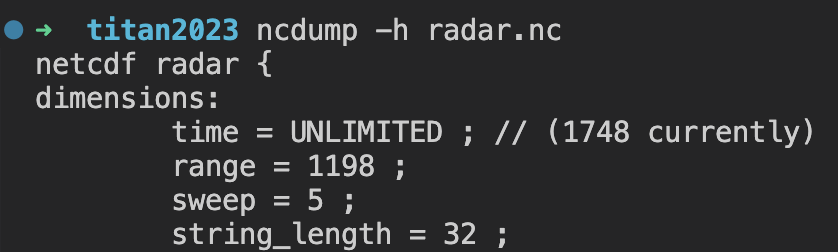
\includegraphics[width=1\linewidth]{Images/ncdump.png}
    \vspace{1em}
    \caption{Radar information in NETCDF format. The total dimensions of the dataset are 2975, grouped into 4 distinct labels.}
    \label{fig:enter-label}
\end{figure}


Foremost among these formats is the Classic Format, which has been a mainstay
since the inception of the NetCDF library and continues to serve as the default
option for file creation. Over time, subsequent releases of the NetCDF library
system have introduced additional formats, each with distinct features tailored
to specific demands. The 64-bit Offset Format, for instance, emerged with
version 3.6.0, addressing the need for expanded variable and file sizes beyond
the limitations of its predecessors.

In a similar vein, the integration of the netCDF-4/HDF5 Format with the release
of version 4.0 represents a milestone in the evolution of the NetCDF ecosystem.
By harnessing the capabilities of the Hierarchical Data Format version 5 (HDF5),
this format bridges the gap between the NetCDF and HDF5 data models, offering
users enhanced capabilities such as support for unlimited dimensions and
substantially larger file sizes. Furthermore, the incorporation of the HDF4 SD
Format and the CDF5 Format underscores the NetCDF ecosystem's commitment to
interoperability and compatibility with parallel processing frameworks.

Central to the design philosophy of NetCDF formats is the concept of
self-description, wherein comprehensive metadata, including attribute name/value
pairs and data array structures, are encapsulated within the file header. This
design not only fosters platform independence but also facilitates seamless data
exchange and interoperability across diverse computational environments.

To illustrate the versatility and efficacy of the NetCDF format, consider a
practical scenario involving the storage of meteorological parameters, including
temperature, humidity, pressure, wind speed, and direction, within NetCDF files.
This exemplifies the format's capacity to accommodate complex, multidimensional
datasets characteristic of scientific research domains, thereby empowering
researchers with a robust and flexible tool for data management and analysis.


Furthermore, it is noteworthy that NetCDF Classic and 64-bit Offset Formats have
garnered international recognition as standards endorsed by the Open Geospatial
Consortium (OGC), underscoring their role as reliable and interoperable
solutions for geospatial data management \cite{ogcnetcdf}. This validation not
only speaks to the robustness and reliability of the NetCDF format but also
underscores its global scalability and compatibility with established standards
and practices in the scientific community.
